% !TEX TS-program = pdflatex
% !TEX encoding = UTF-8 Unicode

% This is a simple template for a LaTeX document using the "article" class.
% See "book", "report", "letter" for other types of document.

\documentclass[11pt]{article} % use larger type; default would be 10pt

\usepackage[utf8]{inputenc} % set input encoding (not needed with XeLaTeX)

%%% Examples of Article customizations
% These packages are optional, depending whether you want the features they provide.
% See the LaTeX Companion or other references for full information.

%%% PAGE DIMENSIONS
\usepackage{geometry} % to change the page dimensions
\geometry{a4paper} % or letterpaper (US) or a5paper or....
% \geometry{margin=2in} % for example, change the margins to 2 inches all round
% \geometry{landscape} % set up the page for landscape
%   read geometry.pdf for detailed page layout information

\usepackage{graphicx} % support the \includegraphics command and options
\usepackage{float} 


% \usepackage[parfill]{parskip} % Activate to begin paragraphs with an empty line rather than an indent

%%% PACKAGES
\usepackage{booktabs} % for much better looking tables
\usepackage{array} % for better arrays (eg matrices) in maths
%\usepackage{paralist} % very flexible & customisable lists (eg. enumerate/itemize, etc.)
\usepackage{verbatim} % adds environment for commenting out blocks of text & for better verbatim
\usepackage{subfig} % make it possible to include more than one captioned figure/table in a single float
% These packages are all incorporated in the memoir class to one degree or another...

%%% HEADERS & FOOTERS
\usepackage{fancyhdr} % This should be set AFTER setting up the page geometry
\pagestyle{fancy} % options: empty , plain , fancy
\renewcommand{\headrulewidth}{0pt} % customise the layout...
\lhead{}\chead{}\rhead{}
\lfoot{}\cfoot{\thepage}\rfoot{}

%%% SECTION TITLE APPEARANCE
\usepackage{sectsty}
\allsectionsfont{\sffamily\mdseries\upshape} % (See the fntguide.pdf for font help)
% (This matches ConTeXt defaults)

%%% ToC (table of contents) APPEARANCE
\usepackage[nottoc,notlof,notlot]{tocbibind} % Put the bibliography in the ToC
\usepackage[titles,subfigure]{tocloft} % Alter the style of the Table of Contents
\renewcommand{\cftsecfont}{\rmfamily\mdseries\upshape}
\renewcommand{\cftsecpagefont}{\rmfamily\mdseries\upshape} % No bold!

%%% END Article customizations

\usepackage[spanish]{babel}
\usepackage{listings} 

%%% The "real" document content comes below...

\title{Documentacion del Proyecto Buscaminas en Android}
\author{Oswaldo Bayona\\Rodrigo Castro\\Jorge Vergara}
%\date{} % Activate to display a given date or no date (if empty),
         % otherwise the current date is printed 

\begin{document}
\maketitle

\section{Introducción}

Your text goes here.

\section{Justificación}



En el desarrollo del proyecto hemos aplicado el paradigma de programación orientado a objetos. Hemos creado varias clases para dividir el problema en pequeñas partes, entre estas clases tememos.
Interface Observer
Esta interface la hemos definido para poder implementar el patrón de diseño Observer, consta de dos eventos Update que sirven para notificar al Observador de los cambios que ocurren en el Observado.

\subsection{Clase Celda}
Esta es una de las clase principales del proyecto simula cada una de las casillas del juego, esta clase extiende de Button e implementa Observer.\\
¿Por qué extiende de Button?\\
Esto se lo hiso principalmente para facilitar el manejo de eventos como click, Drap and Drop utilizando los listener que están definimos para este componente.\\
¿Por qué implementa Observer?\\
Lo hemos implementado así para logran en forma más eficiente el algoritmo para descubrir las celdas, cada celda tiene un ArrayList con sus celdas adyacentes las cuales observan un cambio de esta celda para descubrirse o no dependiendo de la situación, esto involucra que todas las celdas son Observes y a la vez son Observadas por sus adyacentes.
Aparte de estas dos características todas las celdas poseen un estado que puede ser CUBIERTA ,DESCUBIERTA, BANDERA que sirve para que la celda sepa cómo comportarse ante algún evento.\\

\subsection{Clase Tablero}
Esta clase al igual que celda es una de las más importantes, es básicamente un conjunto de celdas que se organizan en forma de matriz, pero hemos decidido utilizar un HaspMap para contener las celdas, porque al no ser muchas celdas se pueden generar muy fácil las claves y el acceso a cada elemento del Mapa es muy rápido, esta clase extiende de View e implementa Observer.\\
¿Por qué se extiende de View?\\
La razón es muy simple el tablero se lo tiene que instanciar dentro de una actividad por lo cual la mejor opción era que extendiera de View\\
¿Por qué se implementa Observer?\\
Básicamente esto es para poder determinar si el juego continúa o finaliza, para esto el Tablero debe observar cuando alguna de las celdas cambie y realizar las validaciones correspondientes.\\

\begin{figure}[H]
 \begin{center}
    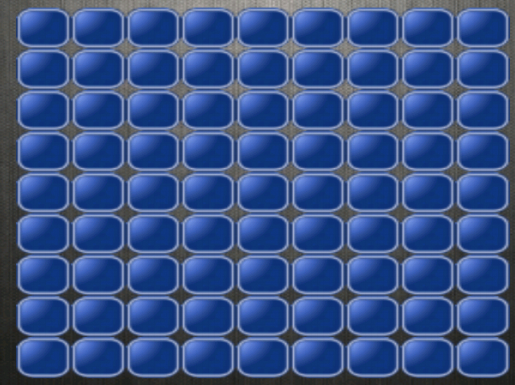
\includegraphics{imagenes_Documentacion/tablero}
\end{center}
\caption {}
\label{Tablero}
\end{figure}


\subsection{Clase Barra de Menu}
Esta clase es muy sencilla consiste en un cronometro, un botón que sirve para reiniciar el juego, una bandera y un contador de banderas, y extiende de TableLayout.\\
¿Por qué extiende de tableLayout?\\
Porque la barra tiene barias componentes y uno forma muy fácil de organizarlos es con el TableLayout.\\

\begin{figure}[H]
 \begin{center}
    
\includegraphics{imagenes_Documentacion/barraMenu}
\end{center}
\caption {}
\label{Barra de Menu}
\end{figure}


\subsection{Comportamiento Drap and Drop}
Se decidió utilizar Drap and Drop porque en Android no existe el Click derecho para poder colocar banderas en una celda, básicamente consiste en poder arrastrar una bandera encima de una celda y luego poder sacar la bandera de la celda arrastrándola.

\begin{figure}[H]
 \begin{center}
    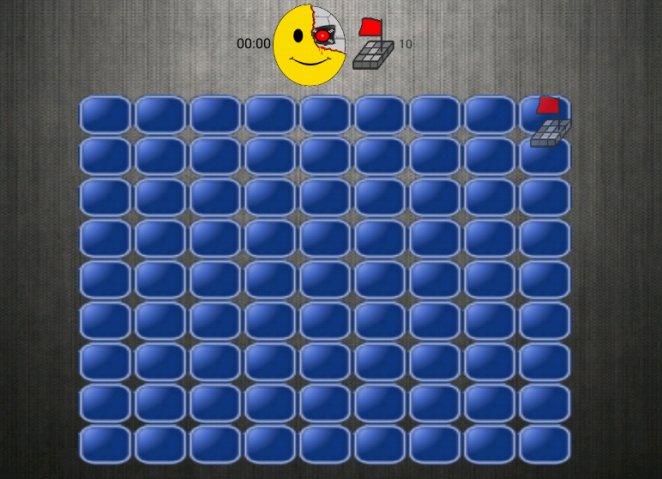
\includegraphics{imagenes_Documentacion/DrapandDrop}
\end{center}
\caption {}
\label{Drap and Drop}
\end{figure}


\subsection{Scroll}
Decidimos utilizar un ScrollView para colocar el tablero porque mientras mayor es el numero de celdas del tablero para que se vean todas las celdas en la pantalla se tendrían que colocar en un tamaño muy pequeño el cual no permitiría jugar al usuario como es debido, esto se soluciono con el scrollView.\\



\section{Alcance}

El proyecto fue escrito en la versión de Android 4.3, con lo cual sólo funcionaría correctamente en dispositivos avanzados.
Nuestro proyecto al inicio  muestra un menú de opciones para elegir entre: Partida Nueva, Acerca De y Top Jugadores, como se muestra en la fig1. La opción Partida Nueva muestra otra actividad para elegir entre tres niveles, Fácil, Intermedio y Experto, la opción de personalizar el número de filas, columnas y bombas del tablero no ha sido implementada. 

\begin{figure}[H]
 \begin{center}
    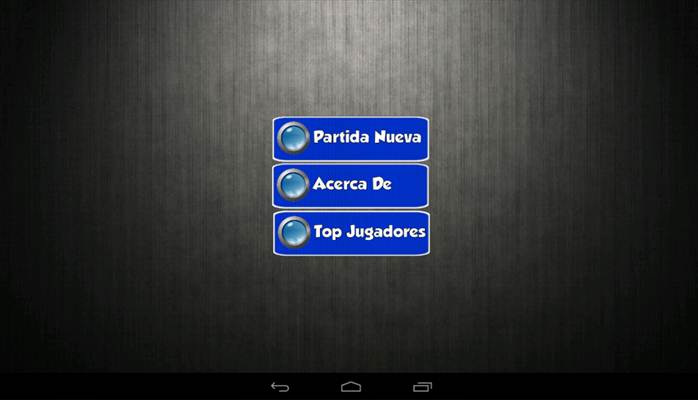
\includegraphics{imagenes_Documentacion/fig1}
\end{center}
\caption {}
\label{Figura 1}
\end{figure}



El tablero del juego muestra básicamente dos Views uno en la parte superior con opciones donde se muestran un cronómetro, un botón para reiniciar el juego, una bandera y un contador; el otro View muestra las celdas.  Los algoritmos recursivos de la expansión de las celdas funcionan muy bien. Todas las opciones  funcionan correctamente, cabe destacar que en el proyecto si fue posible implementar un drag and drop para arrastrar la bandera y ubicarla en la celda, además se puede desde cualquier celda arrastrar la bandera para ser colocada en otra celda o ser eliminada soltándose en un sitio libre de celdas. Fig2

Tenemos implementado varias formas de ganar el juego: una de ellas consiste en descubrir todas las celdas sin minas, pudiendo usar o no usar las banderas; otra manera es que en el momento de haber colocado banderas en todas las celdas con bombas, automáticamente se descubren las celdas que no han sido descubiertas y se gana el juego. Esta última forma se implementó para que el acto de ganar sea más rápido porque el juego también consiste en ganar en el menor tiempo posible y romper records. En el juego existe una cantidad de banderas infinitas, es posible llenar todo el tablero con ellas y seguir arrastrando aunque no haya espacio para ponerlas, en esta situación el contador no es afectado.

\begin{figure}[H]
 \begin{center}
    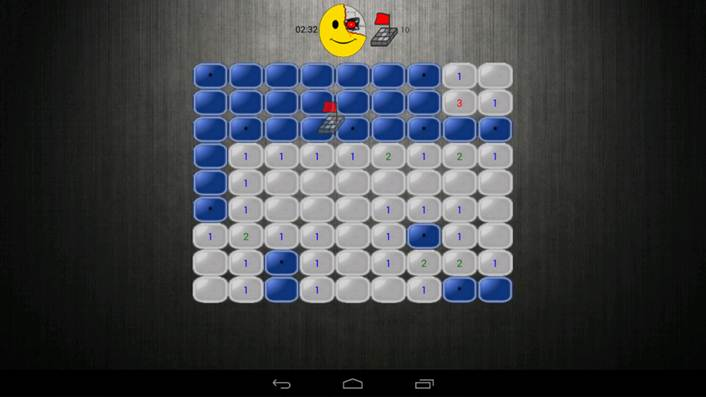
\includegraphics{imagenes_Documentacion/fig2}
\end{center}
\caption {//Tablero del juego: arrastrando una bandera hasta una celda}
\label{Figura 2}
\end{figure}


Al momento de ganar el juego, la aplicación obtiene el tiempo del cronómetro, busca en su base de datos si el tiempo o las condiciones son apropiados para entrar al top. Las condiciones del top son las siguientes, si existen diez o menos jugadores en la lista, se permite el ingreso; si existen más de diez la aplicación revisa si el tiempo es menor a alguno de los existentes y permite el ingreso.  Así como lo implementamos se permite tener infinitos jugadores en la lista.
La base de datos consiste en tres  ficheros .txt (uno para cada nivel) que son guardados en la memoria interna del dispositivo, los datos son presentados al usuario, ordenados de forma descendiente y usando un TableHost para visualizar mejor los resultados.
Entre las cosas que no se pudieron implementar está conseguir mayor portabilidad de la aplicación, no se visualiza bien la resolución en teléfonos o Tablet muy pequeñas, porque fue pensada para funcionar en dispositivos grandes con una resolución de 1280 X 800, tampoco se consiguió que al girar la pantalla del dispositivo la aplicación gire y se adapte a la nueva forma vertical, la aplicación bloque el acelerómetro y mantiene la orientación en horizontal. 







\end{document}
